\section{Basic Distributional Quantities}
\label{sect:dist-quantities}
\begin{enumerate}
\item Here we will introduce some distributional quantities related to a random
variable.  (Some of them are discussed in STAT2901.)
\end{enumerate}
\subsection{Raw and Central Moments}
\begin{enumerate}
\item The \defn{\(k\)th raw moment} (or \(k\)th moment) of a random variable
\(X\), denoted by \(\mu_k'\), is \(\expv{X^k}\).

\begin{note}
The 1st raw moment of a random variable \(X\) is the \emph{mean} of \(X\), and
is denoted by \(\mu\).
\end{note}
\item The \defn{\(k\)th central moment} of \(X\), denoted by \(\mu_k\), is \(\expv{(X-\mu)^k}\).
\item Some quantities of interest related to central moment are as follows.
\begin{center}
\begin{tabular}{ccc}
\toprule
Quantity&Definition&Notation\\
\midrule
\defn{variance}&\(\mu_2\)&\(\sigma^2\)\\
\defn{standard deviation}&\(\sqrt{\mu_2}\)&\(\sigma\)\\
\defn{coefficient of variation}&\(\sigma/\mu\)&\diagbox[dir=NE]{}{}\\
\defn{skewness}&\(\mu_3/\sigma^3\)&\(\gamma_1\)\\
\defn{kurtosis}&\(\mu_4/\sigma^4\)&\(\gamma_2\)\\
\bottomrule
\end{tabular}
\end{center}
\item Here we give interpretations of the quantities not covered in STAT2901:
\begin{itemize}
\item \emph{Coefficient of variation}: It is ``relative'' standard deviation (standard
deviation per unit mean).
\item \emph{Skewness}: It is a measure of \emph{asymmetry}. A symmetric
distribution has a skewness of zero. \begin{warning}
This does \underline{not} mean a distribution with zero skewness is necessarily
symmetric!
\end{warning}
{\color{ForestGreen}Positive} ({\color{red}negative}) skewness indicates
that the {\color{ForestGreen}right} ({\color{red}left}) tail is \emph{longer}
and the mass of distribution is concentrated on the left (right).
\begin{center}
\begin{tikzpicture}
\begin{axis}[domain=-7:7, samples=100, axis lines=middle, xtick=\empty, ytick=\empty, ymin=-0.1, ymax=0.7,
legend entries={positive skewness, negative skewness}, legend style={legend pos=outer north east}]
\addplot[ForestGreen, domain=-5:7]{(-x-5)^2*e^(-x-5)};
\addplot[red, domain=-7:5]{(x-5)^2*e^(x-5)};
\end{axis}
\end{tikzpicture}
\end{center}
\begin{intuition}
Skewness can be written as 
\(\expv{(X-\mu)/\sigma^{3}}\). Since the term inside is raised to
power 3, long right (left) tail contributes very positively (negatively) to
skewness value.
\end{intuition}
\item \emph{Kurtosis}: It measures ``flatness'' of the distribution relative to
a \emph{normal distribution} (which has a kurtosis of 3). When kurtosis is
above (below) 3, it is ``flatter'' (``less flat'') than normal distribution.
(Keeping standard deviation constant, more mass of distribution is located away
from mean, relative to a normal distribution.)
\begin{center}
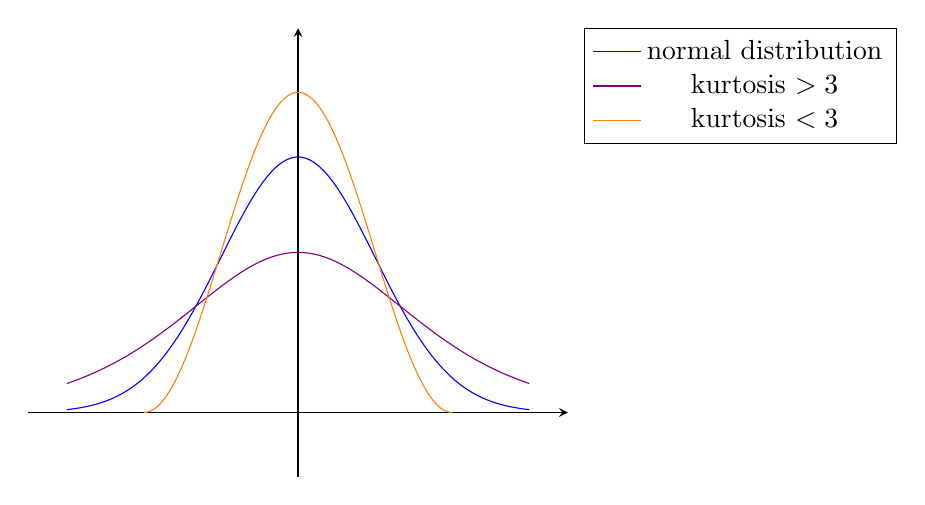
\begin{tikzpicture}
\begin{axis}[domain=-2:2, samples=100, axis lines=middle, xtick=\empty, ytick=\empty, 
xmin=-3.5, xmax=3.5, ymin=-0.1, ymax=0.6,
legend entries={normal distribution, kurtosis \(>3\), kurtosis \(<3\)}, legend style={legend pos=outer north east}
]
\addplot[blue, domain=-3:3]{e^(-x^2/2)/sqrt(2*pi)};
\addplot[violet, domain=-3:3]{e^(-x)/(1+e^(-x))^2};
\addplot[orange]{(1/4)*(1+cos(deg(x*pi/2)))};
\end{axis}
\end{tikzpicture}
\end{center}
\begin{intuition}
Kurtosis can be written as \( \expv{((X-\mu)/\sigma)^{4}}\). Since the term in
the expectation is raised to power 4, mass near mean (with
\((X-\mu)/\sigma<1\)) contributes very little to the kurtosis value, while mass
away from mean (large \((X-\mu)/\sigma\)) contributes a lot to the kurtosis
value.
\end{intuition}
\end{itemize}
\item The following result provides an useful formula for computing mean.
\begin{proposition}
\label{prp:mean-surv}
Let \(X\ge 0\) be a random variable with finite mean (i.e.,
\(\expv{X}<\infty\)), and let \(S_X(x)=\prob{X>x}\) be its survival function. Then,
\[
\expv{X}=\int_{0}^{\infty}S_X(t)\dd{t}.
\]
\end{proposition}
\begin{pf}
Since \(X\ge 0\), we have
\[
X=\int_{0}^{X}1\dd{t}=\int_{0}^{\infty}\indicset{t<X}\dd{t}
\]
\begin{note}
\(\indicset{\cdot}\) denotes the indicator function.
\end{note}

Thus,
\[
\expv{X}=\expv{\int_{0}^{\infty}\indicset{t<X}\dd{t}}
=\int_{0}^{\infty}\expv{\indicset{X>t}}\dd{t}
=\int_{0}^{\infty}\prob{X>t}\dd{t}
\]
where the second equality holds by Fubini's theorem.
\end{pf}

\begin{note}
This result holds no matter \(X\) is discrete or continuous.
\end{note}
\item As a corollary, we have the following the result for \emph{discrete}
random variable.
\begin{corollary}
\label{cor:disc-mean-surv}
Let \(X\) be a discrete random variable with support
\(\N_0\)\footnote{\(\N_0=\{0,1,2,\dotsc\}\)}. Then,
\[
\expv{X}=\sum_{n=0}^{\infty}\prob{X>n}.
\]
\end{corollary}
\begin{pf}
We have
\[
\expv{X}=\int_{0}^{\infty}S_X(t)\dd{t}
=\int_{0}^{1}\underbrace{S_X(t)}_{\prob{X>0}}\dd{t}
+\int_{1}^{2}\underbrace{S_X(t)}_{\prob{X>1}}\dd{t}
+\int_{2}^{3}\underbrace{S_X(t)}_{\prob{X>2}}\dd{t}
+\dotsb
=\sum_{n=0}^{\infty}\prob{X>n}.
\]
\begin{center}
\begin{tikzpicture}
\begin{axis}[domain=0:5, ytick={1, 0,-1,-2, -3, -4},
yticklabels={\(1\), \(\prob{X>0}\), \(\prob{X>1}\), \(\prob{X>2}\),
\(\prob{X>3}\), \(\prob{X>4}\)},
title={\(S_X(t)\)}, xlabel=\(t\)]
\addplot[blue, const plot, jump mark left, mark=*, samples=6]{-x};
\addplot[blue, only marks, mark=o, samples=6]{-x+1};
\draw[very thick, decorate,decoration={calligraphic brace, amplitude=5pt, raise=5pt}] (0,1) -- (0,0)
node[midway, right=0.4cm]{\(\prob{X=0}\)};
\draw[very thick, decorate,decoration={calligraphic brace, amplitude=5pt, raise=5pt}] (1,0) -- (1,-1)
node[midway, right=0.4cm]{\(\prob{X=1}\)};
\draw[very thick, decorate,decoration={calligraphic brace, amplitude=5pt, raise=5pt}] (2,-1) -- (2,-2)
node[midway, right=0.4cm]{\(\prob{X=2}\)};
\draw[very thick, decorate,decoration={calligraphic brace, amplitude=5pt, raise=5pt}] (3,-2) -- (3,-3)
node[midway, right=0.4cm]{\(\prob{X=3}\)};
\end{axis}
\end{tikzpicture}
\end{center}
\end{pf}
\end{enumerate}
\subsection{Stop Loss Variables}
\begin{enumerate}
\item Fix any real number \(d\) and consider a loss \faIcon{fire-alt} random
variable \(X\) (positive value \faIcon{arrows-alt-h} positive loss).  Then, the
\defn{stop loss variable} is 
\[
(X-d)_{+}=\begin{cases}
X-d&\text{if }X> d;\\
0&\text{if }X\le d
\end{cases}
\]
(where \(x_{+}=\max\{x,0\}=x\vee 0\) is the \defn{positive part} of \(x\)).

\item For a practical interpretation of stop loss variable, consider the
following. Suppose that the insurer \faIcon{building} insures a loss \(X\) with
a \defn{deductible} of \(d\) dollars (i.e., the policyholder \faIcon{user}
suffering the loss \(X\) is responsible for first \(d\) dollars of loss, and
\faIcon{building} insures the remaining portion (if exist)). Then, the stop
loss variable represents the payment made by \faIcon{building}:
\begin{itemize}
\item If the loss \(X\le d\), then there is no payment.
\item If the loss \(X>d\), then the payment amount is \(X-d\).
\end{itemize}
\begin{note}
By having such insurance, the policyholder \faIcon{user} suffers \emph{at most}
\(d\) dollars of loss, so the insurance ``stops'' the loss suffered by
\faIcon{user} (from \(d\) dollars onwards) \faIcon{arrow-right} hence ``stop
loss''.
\end{note}

\item \label{it:stop-loss-direct-exp-fmlas}
If \(X\) is continuous with pdf \(f_X\), then
\[
\expv{(X-d)_{+}}=\int_{-\infty}^{\infty}(x-d)_{+}f_X(x)\dd{x}
=\int_{-\infty}^{d}0\dd{x}+\int_{d}^{\infty}(x-d)f_X(x)\dd{x}
=\boxed{\int_{d}^{\infty}(x-d)f_X(x)\dd{x}}.
\]
On the other hand, if \(X\) is discrete, then
\[
\expv{(X-d)_{+}}=\sum_{j}^{}(x_j-d)_{+}\prob{X=j}
=\boxed{\sum_{x_j>d}^{}(x_j-d)\cdot p_j}.
\]
where \(p_j=\prob{X=j}\) and the sum is taken over all \(j\) where \(p_j>0\)
(with \(x_j>d\) for the second sum).

\item We have the following result for the stop loss variable, which is
similar to \cref{prp:mean-surv}.
\begin{proposition}
\label{prp:mean-sl-surv}
Let \(X\) be a (nonnegative or not) random variable with finite mean and let
\(S_X(x)\) be its survival function. Then, for any \(d\in\R\),
\[
\expv{(X-d)_{+}}=\int_{d}^{\infty}S_X(x)\dd{x}.
\]
\end{proposition}
\begin{pf}
Since \((X-d)_{+}\ge 0\) (with finite mean also), by \cref{prp:mean-surv} we have
\[
\expv{(X-d)_{+}}=\int_{0}^{\infty}\prob{(X-d)_{+}>t}\dd{t}
=\int_{0}^{\infty}\prob{X>d+t}\dd{t}
\overset{x=t+d}{=}\int_{d}^{\infty}S_X(x)\dd{x}
\]
where the second equality holds as \((X-d)_{+}>t\iff X>d+t\) for any \(t>0\).
\begin{center}
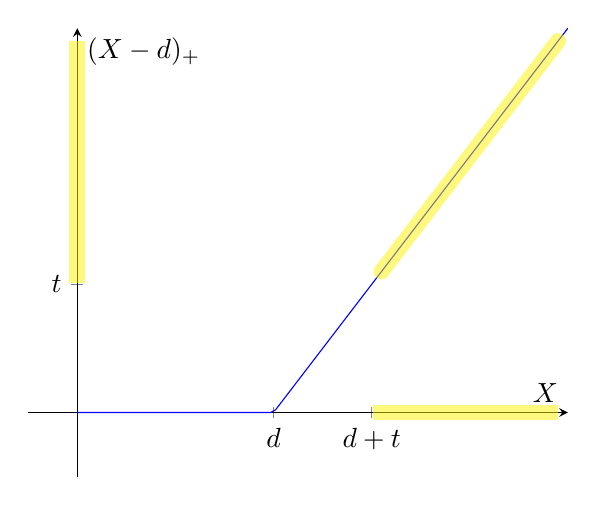
\begin{tikzpicture}[
declare function={sl(\x)=(\x<=2)*0+(\x>2)*(\x-2);}
]
\begin{axis}[domain=0:5,
axis lines=middle, samples=100, xtick={2,3}, xticklabels={\(d\), \(d+t\)}, ytick={1},
yticklabel={\(t\)},
xmin=-0.5, ymin=-0.5, xlabel=\(X\), ylabel=\((X-d)_{+}\)]
\addplot[blue]{sl(x)};
\draw[yellow, opacity=0.5, line width=0.2cm, line cap=round] (3.1,1.1) -- (4.9,2.9);
\draw[yellow, opacity=0.5, line width=0.2cm] (0,1.01) -- (0,2.9);
\draw[yellow, opacity=0.5, line width=0.2cm] (3.01,0) -- (4.9,0);
\end{axis}
\end{tikzpicture}
\end{center}
\end{pf}
\end{enumerate}
\subsection{Excess Loss Variables}
\begin{enumerate}
\item Consider again a loss random variable \(X\) and fix any \(d\in\R\) with
\(\prob{X>d}>0\). Then, the \defn{excess loss variable} (or \defn{residual
lifetime}/``future lifetime random variable for a life aged \(d\)'' (in life
contingencies)) is any random variable \(Y\) with the same distribution
as the conditional distribution of \(X-d\) given \(X>d\), i.e.,
\[
Y\eqd (X-d|X>d).
\]
\item We are usually interested in studying the \emph{expected value} of the
excess loss variable, which is called the \defn{mean excess loss function} (or
\defn{mean residual lifetime} (MRL)/``complete expectation of life'' in life
contingencies):
\[
e_{X}(d)=\expv{Y}=\expv{X-d|X>d}.
\]
\begin{note}
In life contingencies, the actuarial notation is \(\eringx{d}\).
\end{note}
\item \label{it:mrl-fmlas}
If \(X\) is continuous with pdf \(f_X\), then
\[
e_X(d)=\frac{\expv{(X-d)\indicset{X>d}}}{\prob{X>d}}
=\boxed{\frac{\displaystyle\int_{d}^{\infty}(x-d)f_X(x)\dd{x}}{\prob{X>d}}}.
\]
If \(X\) is discrete, then
\[
e_X(d)=\boxed{\frac{\displaystyle \sum_{x_j>d}^{}(x_j-d)p_j}{\prob{X>d}}}
\]
where \(p_j=\prob{X=x_j}\).

\item \label{it:ex-loss-kth-moment-fmlas}
To compute the \(k\)th moment of the excess loss variable \(Y\) (i.e.,
\(\expv{Y^k}\)) (denoted by \(e_X^{k}(d)\)), we can use the following formulas.
\begin{itemize}
\item \(X\) is continuous with pdf \(f_X\):
\[
e_X^{k}(d)=\boxed{\frac{\displaystyle \int_{d}^{\infty}(x-d)^kf_X(x)\dd{x}}{\prob{X>d}}}.
\]
\item \(X\) is discrete:
\[
e_X^{k}(d)=\boxed{\frac{\displaystyle \sum_{x_j>d}^{}(x_j-d)^{k}p_j}{\prob{X>d}}}
\]
where \(p_j=\prob{X=x_j}\).
\end{itemize}
\item \label{it:mrl-exp-sl-relation}
The MRL \(e_X(d)\) and the expected stop loss variable \(\expv{(X-d)_{+}}\) can
be related as follows.
\[
e_X(d)=\frac{\expv{(X-d)\indicset{X>d}}}{\prob{X>d}}
=\frac{\expv{(X-d)\indicset{X>d}+0\cdot\indicset{X\le d}}}{\prob{X>d}}
=\boxed{\frac{\expv{(X-d)_{+}}}{\prob{X>d}}}.
\]
\begin{note}
Using \cref{prp:mean-sl-surv}, we can further write
\[
e_X(d)=\boxed{\frac{\displaystyle \int_{d}^{\infty}S_X(x)\dd{x}}{\prob{X>d}}}.
\]
\end{note}
\end{enumerate}
\subsection{Limited Loss Variables}
\begin{enumerate}
\item Fix any \(u\in\R\) and consider a loss random variable \(X\). Then, the
\defn{limited loss variable} is
\[
X\wedge u=\min\{X,u\}=
\begin{cases}
X&\text{if }X\le u.\\
u&\text{if }X>u;\\
\end{cases}
\]
\item For a practical interpretation of limited loss variable, consider the
following. Suppose that the insurer \faIcon{building} insures a loss \(X\)
with a policy limit of \(u\) dollars (i.e., the maximum loss insured is \(u\)
dollars). Then, the limited loss variable represents the payment made by
\faIcon{building}:
\begin{itemize}
\item If the loss \(X\le u\), then \faIcon{building} pays the full amount \(u\) to
the policyholder \faIcon{user}.
\item If the loss \(X>u\), then \faIcon{building} only pays \(u\) dollars to \faIcon{user}.
\end{itemize}
There is a cap of \(u\) dollars to the payment made by \faIcon{building}.

\item \label{it:lim-loss-kth-moment-fmlas}
To compute the \(k\)th moment of the limited loss variable \(X\wedge u\),
we can use the following formulas.
\begin{itemize}
\item \(X\) is continuous with pdf \(f_X\):
\[
\expv{(X\wedge u)^{k}}=\int_{-\infty}^{\infty}(x\wedge u)^{k}f_X(x)\dd{x}
=\int_{-\infty}^{u}x^kf_X(x)\dd{x}
+\int_{u}^{\infty}u^kf_X(x)\dd{x}
=\boxed{\int_{-\infty}^{u}x^kf_X(x)\dd{x}+u^k\prob{X>u}}.
\]
\item \(X\) is discrete:
\[
\expv{(X\wedge u)^{k}}
=\sum_{j}^{}(x_j\wedge u)^k p_j
=\sum_{x_j\le u}^{}x_j^kp_j+\sum_{x_j>u}^{}u^kp_j
=\boxed{\sum_{x_j\le u}^{}x^kp_j+u^k\prob{X>u}}
\]
where \(p_j=\prob{X=x_j}\).
\end{itemize}
\item \label{it:sl-limloss-relation}
Stop loss and limited loss variables can be related as follows. For any
\(d\in\R\) and any random variable \(X\),
\[
(X-d)_{+}+(X\wedge d)=X.
\]
\begin{pf}
We have
\[
{\color{violet}(X-d)_{+}}+{\color{orange}(X\wedge d)}
=\begin{cases}
{\color{violet}X-d}+{\color{orange}d}&\text{if }X>d;\\
{\color{violet}0}+{\color{orange}X}&\text{if }X\le d
\end{cases}
=X.
\]
\begin{center}
\begin{tikzpicture}[
declare function={
sl(\x)=(\x<=2)*0+(\x>2)*(\x-2);
ll(\x)=(\x<=2)*\x+(\x>2)*2;
}
]
\begin{axis}[domain=0:5,
axis lines=middle, samples=100, xtick={2}, xticklabels={\(d\)}, 
ytick={2}, yticklabels={\(d\)},
xmin=-0.5, ymin=-0.5, xlabel=\(X\) ,legend entries={\((X-d)_{+}\), \(X\wedge d\), \(X\)}
,legend style={legend pos=outer north east}]
\addplot[violet, dashed, thick]{sl(x)};
\addplot[orange, dashed, thick]{ll(x)};
\addplot[blue]{sl(x)+ll(x)};
\end{axis}
\end{tikzpicture}
\end{center}
\end{pf}

\begin{note}
A practical interpretation of this result is that combining an insurance with
deductible \(d\) and another insurance with policy limit \(d\) gives an
insurance with full coverage.
\end{note}
\item Due to the relationship in \labelcref{it:sl-limloss-relation}, we can
obtain the following formula for computing expected limited loss (assuming
\(X\) has finite mean and is nonnegative), using
\cref{prp:mean-surv,prp:mean-sl-surv}:
\[
\expv{X\wedge u}=\expv{X}-\expv{(X-u)_{+}}
=\int_{0}^{\infty}S_X(x)\dd{x}-\int_{u}^{\infty}S_x(x)\dd{x}
=\boxed{\int_{0}^{u}S_X(x)\dd{x}}.
\]
where \(S_X\) is the survival function of \(X\).
\end{enumerate}
\subsection{Comparing Tail Thickness of Distributions}
\begin{enumerate}
\item An important consideration in risk management for an insurer
\faIcon{building} is to properly quantify the ``thickness'' of the right tail
of distribution of loss \(X\) since it can greatly impact the financial
position of \faIcon{building}. The higher probability assigned to extremely
large values, the ``thicker''/``heavier'' the right tail.

\begin{center}
\begin{tikzpicture}
\begin{axis}[domain=-5:5, samples=100, axis lines=middle, xtick=\empty, ytick=\empty, 
xmin=-5.5, xmax=5.5, ymin=-0.1, ymax=0.5,
legend entries={thinner tails, thicker tails}, legend style={legend pos=outer north east}
]
\addplot[green]{e^(-x^2/2)/sqrt(2*pi)};
\addplot[red]{1/(pi*(1+x^2))};
\end{axis}
\end{tikzpicture}
\end{center}
\item To \emph{compare} tail thickness, we can consider the following methods:
\begin{enumerate}
\item comparison based on existence and non-existence of moments
\item comparison based on limit of ratio of survival functions
\item comparison based on hazard rate function (``force of mortality'' in life contingencies)
\item comparison based on MRL (or mean excess loss function)
\end{enumerate}
\begin{note}
Here we focus on continuous random variables. But the methods can also be used
for discrete random variables in a similar manner.
\end{note}
\item First we consider comparison based on moments. Here we focus on a
nonnegative loss \(X\). Recall that the \(k\)th raw moment of \(X\) with pdf
\(f_X\) is
\[
\mu_k'=\expv{X^k}=\int_{-\infty}^{\infty}x^kf_X(x)\dd{x}
\]
If \(f_X(x)\) is relatively large for large \(x\), it indicates that \(X\) has
a relatively thick right tail. Hence, a method for assessing tail thickness is
to check the \emph{speed} of \(f_X(x)\to 0\) as \(x\) rises.

When the \(k\)th moment \(\expv{X^k}\) exists/is finite (i.e.,
\(\expv{X^k}<\infty\)), it suggests that \(f_X(x)\to 0\) \emph{much faster} than the
speed at which \(x^k\to\infty\) \faIcon{arrow-right} lighter right tail.

On the other hand, if it is infinite (i.e., \(\expv{X^k}=\infty\)), then it
indicates that \(f_X(x)\to 0\) \emph{much slower} than the speed at which
\(x^k\to\infty\) \faIcon{arrow-right} thicker right tail.

\item Regarding the existence/non-existence of moments, we have the following
result.
\begin{proposition}
\label{prp:high-low-moment-relation}
Suppose that \(X\) is a nonnegative random variable. Fix any \(r,k>0\) with
\(0<r<k\). Then,
\[
\expv{X^k}<\infty\implies \expv{X^r}<\infty.
\]
(So, existence of \(k\)th moment implies existence of
all smaller positive moments.)

\begin{note}
Equivalently,
\[
\expv{X^r}=\infty\implies \expv{X^k}=\infty.
\]
(So, non-existence of \(r\)th moment implies non-existence of
all larger positive moments.)
\end{note}
\end{proposition}
\begin{pf}
Assume that \(\expv{X^k}<\infty\). Then,
\begin{align*}
\expv{X^r}&=\expv{X^r\indicset{0\le X\le 1}}+\expv{X^r\indicset{X>1}}\\
&\le \expv{\indicset{0\le X\le 1}}+\expv{X^k\indicset{X>1}} &\text{(\(X^r \le 1\) when \(0\le X\le 1\), and \(X^r\le X^k\) when \(X>1\))}\\
&\le \expv{\indicset{0\le X\le 1}}+\expv{X^k}&\text{(\(\indicset{X>1}\le 1\) and \(X^k\ge 0\))}\\
&=\prob{0\le X\le 1}+\expv{X^k}\\
&<\infty.
\end{align*}
\end{pf}

Hence, if it is not the case that \(X\) has finite \(k\)th moment for any
\(k>0\), then we can find a ``turning point'' \(k^*>0\) at which the moment
changes from finite to infinite, i.e.,
\[
\expv{X^k}<\infty\;\forall 0<k< k^*\qqtext{and}
\expv{X^k}=\infty\;\forall k\ge k^*.
\]
\begin{center}
\begin{tikzpicture}
\draw[-Latex] (0,0) -- (10,0);
\filldraw[blue] (4,0) circle [radius=0.3mm]
node[above]{\(k^*\)};
\draw[very thick, decorate,decoration={mirror, calligraphic brace, amplitude=5pt, raise=5pt}] (0,0) -- (3.95,0)
node[midway, below=0.4cm]{\(\expv{X^k}<\infty\)};
\draw[very thick, decorate,decoration={mirror, calligraphic brace, amplitude=5pt, raise=5pt}] (4,0) -- (9.8,0)
node[midway, below=0.4cm]{\(\expv{X^k}=\infty\)};
\end{tikzpicture}
\end{center}
\item Thus, we have the following indicators for tail thickness:
\begin{itemize}
\item Existence of \(k\)th moment for any \(k>0\) \faIcon{arrow-right} ``rather light'' right tail.
\item Between two nonnegative losses \(X\) and \(Y\), if the ``turning point''
of \(X\) is smaller than that of \(Y\), then \(X\) has a \emph{thicker} right
tail than \(Y\). \begin{note}
To see this, note that in this case we can find a \(k>0\) such that
\(\expv{X^k}=\infty\) and \(\expv{Y^k}<\infty\), which means that \(f_X(x)\to
0\) \emph{much slower} than \(x^k\to\infty\), while \(f_Y(x)\to 0\) \emph{much faster}
than \(x^k\to\infty\) \faIcon{arrow-right} \(f_X(x)\to 0\) \emph{much slower} than
\(f_Y(x)\to 0\) \faIcon{arrow-right} \(X\) has a \emph{thicker} right tail than
\(Y\).
\end{note}
\end{itemize}
\item Now we consider comparison based on limit of ratio of survival functions.
To compare the tail thickness between \(X\) and \(Y\), we consider the limit
\[
\lim_{t\to \infty}\frac{S_X(t)}{S_Y(t)}
\]
where \(S_X\) and \(S_Y\) are survival functions of \(X\) and \(Y\) respectively.

Suppose the limit is \(c\) (which may be \(\infty\)). Then, we can compare the
tail thickness based on \(c\):
\begin{itemize}
\item \(c=0\): \(S_X(t)\to 0\) \emph{much faster} than \(S_Y(t)\to 0\) as \(t\to\infty\)
\faIcon{arrow-right} \(Y\) has a \emph{thicker} right tail than \(X\)
\item \(0<c<\infty\): \(S_X(t)\to 0\) at a ``similar'' speed to \(S_Y(t)\to 0\)
as \(t\to\infty\) \faIcon{arrow-right} \(X\) and \(Y\) have ``similar'' right
tail thickness
\item \(c=\infty\): \(S_X(t)\to 0\) \emph{much slower} than \(S_Y(t)\to 0\) as \(t\to\infty\)
\faIcon{arrow-right} \(X\) has a \emph{thicker} right tail than \(Y\)
\end{itemize}
\begin{note}
When \(S_X(t)\) is relatively large for large \(t\), it suggests that
relatively high probability is assigned to large values \faIcon{arrow-right}
relatively thick right tail.
\end{note}

\item \label{it:lim-surv-ratio-equal-lim-pdf-ratio}
To compute the limit \(\displaystyle \lim_{t\to \infty}\frac{S_X(t)}{S_Y(t)}
\), we can apply the L'H\^{o}pital's rule:
\[
\lim_{t\to \infty}\frac{S_X(t)}{S_Y(t)}
=\lim_{t\to \infty}\frac{S_X'(t)}{S_Y'(t)}
=\boxed{\lim_{t\to \infty}\frac{f_X(t)}{f_Y(t)}}.
\]
where \(f_X\) and \(f_Y\) are pdfs of \(X\) and \(Y\) respectively.

\item Next, we consider the comparison based on hazard rate
function. The \defn{hazard rate function} of a random variable \(X\) is
\[
h_X(x)=\frac{f_X(x)}{S_X(x)}
\]
where \(f_X\) and \(S_X\) are pdf and survival function of \(X\) respectively.

\begin{note}
It is ``force of mortality'' in life contingencies.
\end{note}

To interpret the hazard rate, note that
\[
\prob{x<X\le x+h|X>x}=\frac{\prob{x<X\le x+h}}{S_X(x)}
\approx\frac{f(x)h}{S_X(x)}=h_X(x)h
\]
for small \(h\). Thus, in infinitesimal, \(h_X(x)\dd{x}\) gives the probability
that \(X\in(x,x+\dd{x}]\) (``failing instantaneously'') given \(X>x\) (``surviving'').
Hence, the hazard rate can be regarded as \emph{instantaneous failure rate}.

\item To assess the tail thickness based on hazard rate function, consider the
following.
\begin{itemize}
\item If \(h_X(x)\) is a decreasing (or non-increasing) function, then for
larger \(x\), given \(X>x\), it is \emph{less} likely for \(X\in(x,x+\dd{x}]\)
and hence \emph{more} likely for \(X>x+\dd{x}\) (higher probability for
\emph{even larger} \(x\)) \faIcon{arrow-right} \(X\) has a thick right tail.

\item If \(h_X(x)\) is an increasing (or non-decreasing) function, then for
larger \(x\), given \(X>x\), it is \emph{more} likely for \(X\in(x,x+\dd{x}]\)
and hence \emph{less} likely for \(X>x+\dd{x}\) (lower probability for
\emph{even larger} \(x\)) \faIcon{arrow-right} \(X\) has a light right tail.
\end{itemize}
\begin{note}
Here ``less'' and ``more'' likely are in a non-strict sense: They also include
the case ``as likely''.
\end{note}
\item A random variable \(X\) has \defn{decreasing failure rate} (DFR) if
\(h_X(x)\) is decreasing in \(x\), and has \defn{increasing failure rate} (IFR)
if \(h_X(x)\) is increasing in \(x\).

Hence, \(X\) has thick (light) right tail if \(X\) has DFR (IFR).

\item Lastly, we consider the comparison based on mean residual lifetime (MRL).
\begin{itemize}
\item If \(e_X(d)\) is decreasing in \(d\), then it suggests that there is not
much excess loss (on average) once \(d\) is large \faIcon{arrow-right} not much
probability is assigned to large \(x\) \faIcon{arrow-right} \(X\) has a light
right tail.

\item If \(e_X(d)\) is increasing in \(d\), then it suggests that there is
still more excess loss (on average) when \(d\) gets larger \faIcon{arrow-right}
quite a lot of probability is assigned to large \(x\) \faIcon{arrow-right}
\(X\) has a heavy right tail.
\end{itemize}

\item A random variable \(X\) has \defn{decreasing mean residual lifetime} (DMRL) if
\(e_X(d)\) is decreasing in \(d\), and has \defn{increasing mean residual
lifetime} (IMRL) if \(e_X(d)\) is increasing in \(d\).

Hence, \(X\) has thick (light) right tail if \(X\) has IMRL (DMRL).

\item Naturally, one would then be interested in the relationship between
DFR/IFR and DMRL/IMRL. This is given as follows.
\begin{proposition}
\label{prp:fr-imp-inv-mrl}
Let \(X\) be a random variable. Then,
\[
\text{\(X\) has DFR \(\implies\) \(X\) has IMRL}
\qqtext{and}
\text{\(X\) has IFR \(\implies\) \(X\) has DMRL}.
\]
\end{proposition}
\begin{pf}
Firstly, since
\[
h_X(x)=\frac{f_X(x)}{S_X(x)}=-\dv{}{x}\ln S_X(x),
\]
we have
\[
S_X(x)=\exp(-\int_{-\infty}^{x}h_X(y)\dd{y}),
\]
so
\[
\frac{S_X(x+t)}{S_X(x)}=\exp(-\int_{x}^{x+t}h_X(y)\dd{y})
=\exp(-\int_{0}^{t}h_X(x+y)\dd{y}).
\]
\begin{note}
The formula corresponding to this in life contingencies is
\(S_x(t)=\exp(-\int_{0}^{t}\mu_{x+s}\dd{s})\).
\end{note}

Now, assume \(X\) has DFR and fix any \(t\ge 0\). Then, from the equation above
we know \(\displaystyle \frac{S_X(x+t)}{S_X(x)}\) is increasing in \(x\). Thus,
by \labelcref{it:mrl-exp-sl-relation}, for any \(d_1\le d_2\),
\[
e_X(d_1)=\frac{\displaystyle \int_{0}^{\infty}S_X(d_1+t)\dd{t}}{S_X(d_1)}
=\int_{0}^{\infty}\frac{S_X(d_1+t)}{S_X(d_1)}\dd{t}
\le \int_{0}^{\infty}\frac{S_X(d_2+t)}{S_X(d_2)}\dd{t}
=e_X(d_2),
\]
meaning that \(e_X(d)\) is increasing in \(d\), so \(X\) is IMRL.

Proof of another implication is similar.
\end{pf}

\begin{warning}
The converse implications are \underline{not} true. That is,
\[
\text{\(X\) has IMRL \(\centernot\implies\) \(X\) has DFR}
\qqtext{and}
\text{\(X\) has DMRL \(\centernot\implies\) \(X\) has IFR}.
\]
\end{warning}
\end{enumerate}
